\documentclass[11pt, twocolumn]{article} 
\def\name{\note{MY NAME}}
\def\doctitle{\note{DOCUMENT TITLE}}
\def\subjectcode{\note{SUBJECT CODE}}
\def\studentnumber{\note{STUDENT NUMBER}}
% Geometry and Layout
    \usepackage[margin=0.75in]{geometry}
    \usepackage{parskip}
    \usepackage{placeins} % FloatBarrier

% Font
    \usepackage[T1]{fontenc}      
    \usepackage{fourier}          % sick font

% inline typsetting of units and quantities
    \usepackage{siunitx}
% Graphics and Diagrams
    \usepackage{wrapfig}

    \usepackage{xcolor}
    \usepackage{graphicx} % Required for inserting images
    \usepackage[american]{circuitikz}
    \usepackage{tikz}
    \usepackage{tikz-3dplot}
    \usetikzlibrary{arrows.meta}
    \usetikzlibrary{positioning}  % Add this line to load the positioning library
    \usepackage{pgfplots}
    \pgfplotsset{compat=newest}
    \usepackage{listings}
    \usepackage{tcolorbox}

% CSV Table input
    \usepackage[table]{xcolor}
    \usepackage{csvsimple, booktabs}

% Code Chunk Formatting
    \definecolor{comment_color}{rgb}{0.52,0.38,0.78}
    \definecolor{keyword_color}{rgb}{0.84,0.27,0.3}
    \definecolor{background_color}{rgb}{0.95,0.95,0.95}
    \usepackage{inconsolata} % Consolas-style font from the inconsolata package

\lstset{
    backgroundcolor=\color{background_color},   % Choose the background color
    commentstyle=\color{comment_color},       % Style of comments
    keywordstyle=\color{keyword_color},        % Style of keywords
    stringstyle=\color{red},              % Style of strings, assuming red
    basicstyle=\tiny\ttfamily, % Set font size, monospaced font, and color        
    breakatwhitespace=false,              % Automatic line breaking only at whitespace
    breaklines=true,                      % Automatic line breaking
    captionpos=t,                         % Caption position is on top
    keepspaces=true,                      % Keeps spaces in text
    numbers=left,                         % Line number position
    numbersep=5pt,                        % How far the line numbers are from the code
    showspaces=false,                     % Show spaces in the code
    showstringspaces=false,               % Underline spaces within strings only
    showtabs=true,                       % Show tabs within strings adding particular underscores
    % framexleftmargin=5pt,                       % Extra space on the left for better aesthetics
    xleftmargin=0.05\textwidth,                 % Indent from the left
    xrightmargin=0.05\textwidth,                % Indent from the right
    tabsize=1,                            % Sets default tab size
    title=\lstname                        % Show the filename of files included with \lstinputlisting
}
% Text Content / Math
    \usepackage{lipsum} % Dummy text
    \usepackage{hyperref}
    \usepackage{amsmath} % For sum symbol and other math formatting
    \usepackage{amssymb}

% Headers and Footers
    \usepackage{lastpage}
    \usepackage{fancyhdr}
    \makeatletter
    \renewcommand{\@seccntformat}[1]{}
    \makeatother
    \pagestyle{fancy}
    \fancyhf{} 
    \setlength{\headheight}{15pt}
    \fancyhead[L]{\subjectcode{} - \doctitle{}}
    \fancyhead[R]{} % Rearrange as you please
    \fancyfoot[L]{\name{}}
    \fancyfoot[R]{Page \thepage\ of \pageref{LastPage}} 
    \renewcommand{\headrulewidth}{0pt}

% Caption and Referencing Customization
    \usepackage[justification=centering]{caption}
    \usepackage{cleveref}
    \usepackage{nameref}
    \DeclareCaptionLabelSeparator{IEEE}{.\quad }
    \captionsetup[figure]{name=Fig., labelsep=IEEE}
    \captionsetup{format=hang, labelfont=bf}
    \captionsetup{justification=raggedright,singlelinecheck=false}

% Document Metadata and First Page Formatting
    \title{\doctitle{}\\\large{James Cook University Cairns}}
    \author{\name{} (\studentnumber{})}
    \date{\today}

% Referencing
    \usepackage[noadjust]{cite} % For IEEE-style citations
    \renewcommand{\refname}{} % Remove "References" title

\newcommand{\codeblock}[4]{
    \lstinputlisting[language=#1, caption={#2}, label=#3]{#4}
} %command for inserting code blocks because im a G


\newcommand{\E}[1]{
    \cdot 10^{#1}
} % way easier to type

\newcommand{\abs}[1]{
    \left\lvert #1 \right\rvert
} % feels like it should be a command by default to be honest

\newcommand{\note}[1]{\textcolor{red}{#1}} %create a red note for yourself


\definecolor{codegray}{gray}{0.9} % Light gray color
\newcommand{\code}[1]{\colorbox{codegray}{\texttt{\detokenize{#1}}}} % Command for inline code


%Choose which files are re-rendered (saves rendering time)
%\includeonly{}

\begin{document}
    % Create the title page
    \begin{titlepage}
        \maketitle
        \thispagestyle{empty} %suppresses page numbering on the title page
    \end{titlepage}

    % Table of Contents
    \thispagestyle{empty} % Suppresses page numbering on the contents page
    \onecolumn
    \tableofcontents
    \listoffigures
    \listoftables
    \twocolumn % get rid of this line if you prefer one column report

    \clearpage
    \section{Intro}

This is my cool document. I have a lot of cool things to say. \note{note to self: Improve this introduction}. These papers say something that i agree with \cite{normal_distribution_wiki_page,latex_project_website}. Also have a look at \cref{code:python_code,fig:circuit_Diagram,fig:sick_graphs}.

\begin{figure}[ht]
    \centering
    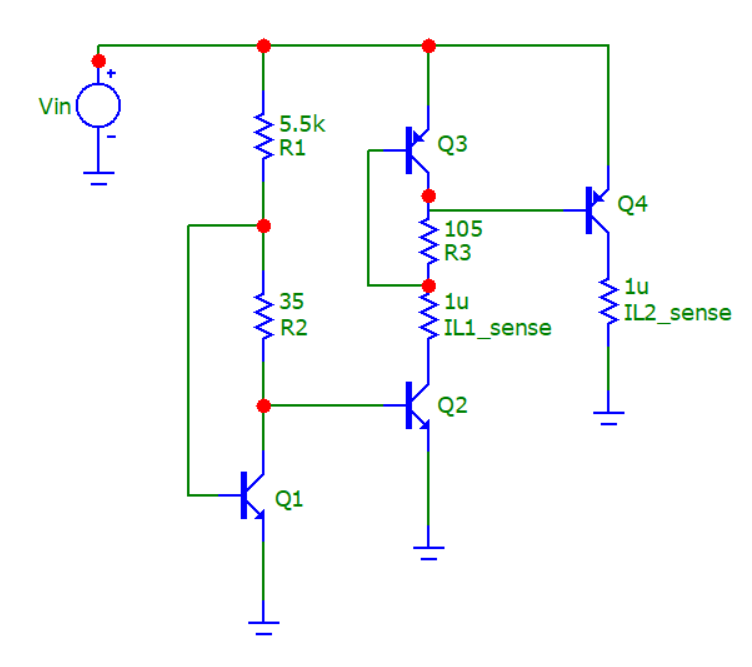
\includegraphics[width=\linewidth]{figures/c3.png} % Image filename
    \centering
    \caption{Circuit Diagram} % Caption
    \label{fig:circuit_Diagram} % Label
\end{figure}

\begin{figure*}[ht]
    \centering
    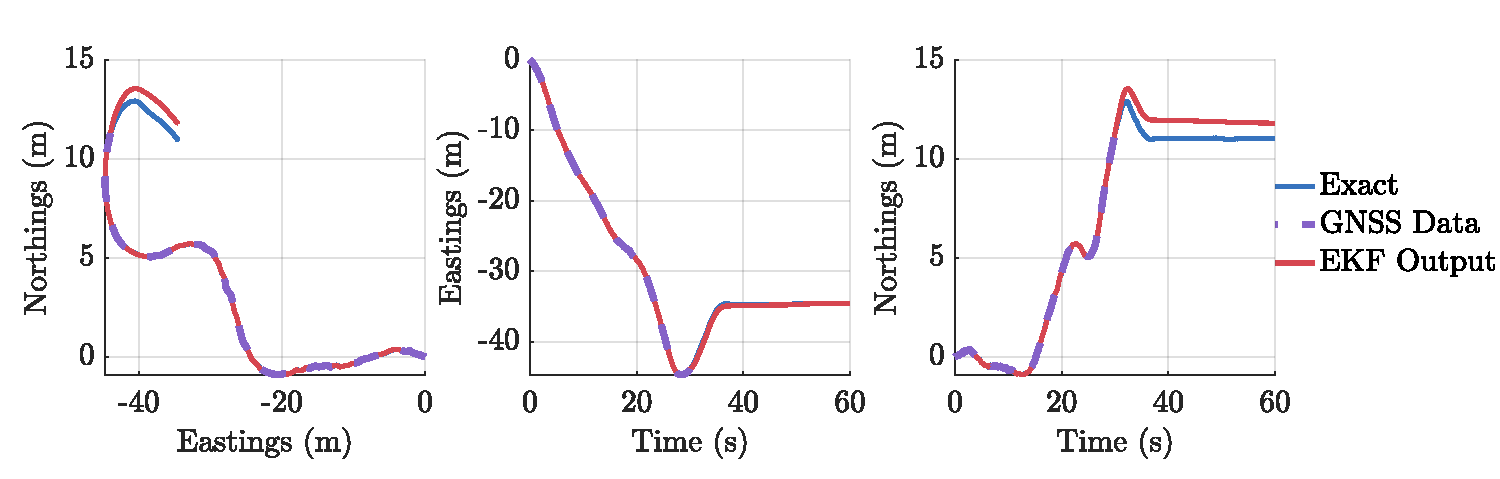
\includegraphics[width=\linewidth]{figures/R6.pdf} % Image filename
    \centering
    \caption{Sick Graphs} % Caption
    \label{fig:sick_graphs} % Label
\end{figure*}


\lstinputlisting[language=Python, caption=Python code, label=code:python_code]{../code/python.py}

\begin{table}[ht]
    \centering
    \begin{tabular}{ccccc}
        \toprule
        \textbf{recording} & 
        \textbf{mean $\Delta \vec{p}$} & 
        \textbf{final $\Delta \vec{p}$} & 
        \textbf{max $\Delta \vec{p}$} \\
        \midrule
        \csvreader[head to column names, late after line=\\]{../data/data.csv}{}
        {\csvcoli & \csvcolii & \csvcoliii & \csvcoliv}
        \bottomrule
    \end{tabular}
    \caption{Summary statistics read from \code{../data/data.csv}}
    \label{table_from_file}
\end{table}




    %\input{sec_2_content.tex}
    %\input{sec_3_content.tex}

    % bibliography at the end
    %\clearpage % uncomment if you want the references on a new page
    \onecolumn % uncomment if you want the references in one column

    \bibliographystyle{ieeetran}
    \section{References}  % This creates a numbered section heading for References
    \bibliography{references.bib}

\end{document}